%%%%%%%%%%%%%%%%%%%%%%%%%%%%%%%%%%%%%%%%%%%%%%%%%%%%%%%%%%%%%%
%% Made by Nirmal Iyer
%% Document on LAXPC pointing for observations of 1E source by graman
%% First made - Mon 11 Dec 2017 05:04:39 PM CET 
%--------------------
%% 1. First draft - Nirmal 
%%%%%%%%%%%%%%%%%%%%%%%%%%%%%%%%%%%%%%%%%%%%%%%%%%%%%%%%%%%%%%%%
% article example for classicthesis.sty
\documentclass[11pt,a4paper,eulermath,pdfspacing]{article} % KOMA-Script article scrartcl
%\usepackage{lipsum}
\usepackage{url}
\usepackage[nochapters,]{classicthesis} % nochapters
\usepackage{natbib}
\usepackage{enumitem}
\usepackage{subfig}
\usepackage{graphicx}
\hypersetup{urlcolor=webbrown,linkcolor=RoyalBlue,citecolor=webgreen,colorlinks=true, linktocpage=true}
\usepackage{listings}
\lstset{
language=Python,
basicstyle=\small\ttfamily,
otherkeywords={self,calcarea,Collimator},             % Add keywords here
keywordstyle=\color{RoyalBlue},
emph={pt2d,Collimator,__init__},          % Custom highlighting
emphstyle=\ttfamily\color{webbrown},    % Custom highlighting style
stringstyle=\rmfamily,
frame=single,                         % Any extra options here
frameround=ftfff,
commentstyle=\color{webgreen}\ttfamily
%showstringspaces=true            % 
}


% ********************************************************************
% Changing the text area
% ********************************************************************
\linespread{1.15} % a bit more for Palatino
\areaset[current]{468pt}{761pt} % 686 (factor 2.2) + 33 head + 42 head \the\footskip
\setlength{\marginparwidth}{1.1em}%
\setlength{\marginparsep}{1em}%

\newcommand\mydeg{\ifmmode ^{\circ} \else $^{\circ}$\fi}
\newcommand\arcsec{\hbox{$^{\prime\prime}$}}
\newcommand\arcmin{\hbox{$^{\prime}$}}


\begin{document}
	\title{\spacedlowsmallcaps{LAXPC pointing for 1E 1743.1-2843}}
	\author{\spacedlowsmallcaps{\today}}
	\date{Version 1.0} 
    \maketitle
%\section*{Version History}
%\begin{itemize}
%  \item Version 1 : Made on 07 Jun 2017. First basic version of	document. Author - Nirmal
%  \item Version 1.1 : Made on 09 Jun 2017. Added details for shielding
%	considerations. Author - Nirmal
%\end{itemize}
 
\section{Introduction}
This document elaborates the procedure used to determine pointing directions for
each of the LAXPCs when the possible thermonuclear burst in 1E 1743.1-2843 was
detected.

\section{Calculation of LAXPC pointing}
The pointing direction of each of the three different LAXPCs are computed from
the ROLL pointing of AstroSat. The ROLL pointing is obtained from the attitude
file. The offset from ROLL pointing is obtained using data from Table 2 of the LAXPC calibration paper
\citep{anti:2017}. 

This table gives the pointing offsets of each LAXPC from the
ROLL pointing direction of Crab. However, it does not mention the orientation
(attitude) of the satellite (viz. the pointing direction of the YAW and PITCH
axes). Thus, the given offsets can be in any direction from a new pointing of
AstroSat with the offset magnitude being the same. This gives a circle of
possible LAXPC pointings around the AstroSat ROLL pointing. The points of the
circle can be computed in two ways as mentioned in the following subsection.

\subsection{Uncertainty in offsets}
Two methods can be used to compute the LAXPC pointing from a given AstroSat
pointing direction.
\begin{enumerate}
	\item The immediately apparent method uses the offset angle $\theta_{offs}$
		given for each LAXPC with the ROLL pointing to find the locus of points
		satisfying this criterion. If ROLL pointing is given by angles RA
		($\alpha_1$) and Dec ($\delta_1$), then the locii of points
		($\alpha_2$, $\delta_2$) are found from the equation for angular distance
		\begin{equation}
			cos(\theta_{offs}) = \sin{\delta_1}\sin{\delta_2} +
			\cos{\delta_1}\cos{\delta_2}\cos{(\alpha_1 - \alpha_2)}
			\label{eqn:diff}
		\end{equation}

\begin{figure}[!h]
  \centering
  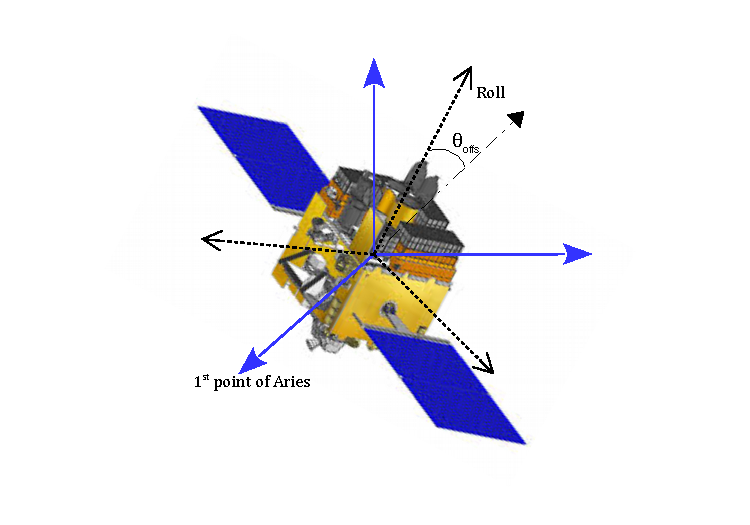
\includegraphics[width=0.8\textwidth]{./AstroSat_pntng.pdf}
  \caption{AstroSat pointing direction and the co-ordinate systems. Blue axes
  coraxes correspond to the inertial co-ordinate system and black axes to the
  satellite body co-ordinate system.}
  \label{fig:coord}
\end{figure}


	\item The second method uses transformation between the satellite body
		co-ordinate system (in which the ROLL, YAW , PITCH and LAXPC directions
		are defined) and inertial co-ordinate system ( in which RA and Dec are
		defined). The co-ordinate axes are illustrated in \autoref{fig:coord}. 
		The advantage of using this method is the that it can give an exact
		pointing direction for each LAXPC if the ROLL, PITCH and YAW directions
		of the Crab observations used for making Table 2 of the calibration
		paper are known. This method is based on the co-ordinate transformation
		formulations used in the SSM, CZTI and SXT imaging detectors
		\citep{dip1,dip2}.

\begin{figure}[!b]
	\centering
	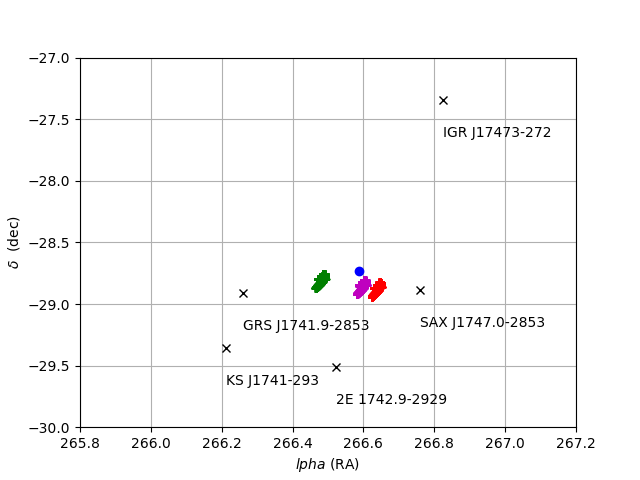
\includegraphics[width=0.7\textwidth]{./1st_try.png}
	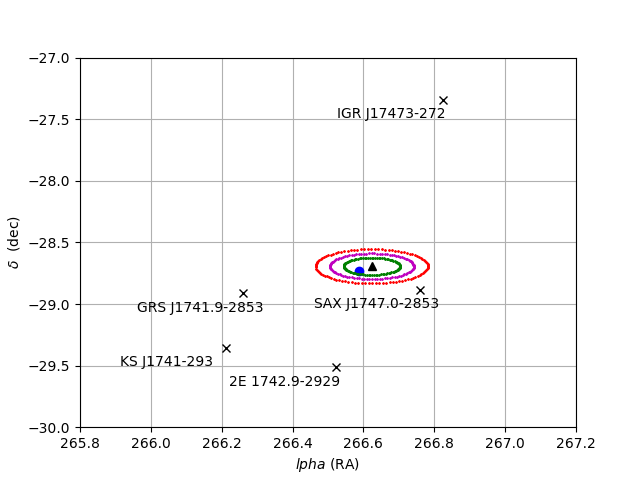
\includegraphics[width=0.7\textwidth]{./2nd_try.png}
	\caption{Offset plots for the bursting observation. Blue circle is 1E
	1743.1-2843. Black triangle is AstroSat pointing. Red is LAXPC10, Green is
	LAXPC20 and Magenta is LAXPC30 pointing.}
	\label{fig:fixvar}
\end{figure}



		The steps for this method are given below :
		\begin{itemize}
			\item Get the quaternion $q_{pnt}$ for satellite pointing during the
				burst. From this obtain the rotation matrix $R_{b2i}$ for converting from
				satellite body to inertial co-ordinates.
			\item Get the quaternion $q_{cr}$ for the satellite pointing of the Crab for
				which LAXPC offset calibrations were made. From this obtain the
				rotation matrix $R^{fix}_{i2b}$ for shifting the offset
				$\theta_{offs}$ from inertial to satellite body co-ordinates.
			\item If $q_{cr}$ is not available, construct a set of
				$R^{var}_{i2b}$ from using ROLL along Crab RA, Dec and YAW,
				PITCH in different positions perpendicular to the ROLL.
			\item Shift the offset from inertial to body co-ordinates. This is
				done by computing the LAXPC pointing in satellite body
				co-ordinates as 
				\begin{equation}
					lxpc_{body} = R_{i2b} * lxpc_{inert}
					\label{eqn:i2b}
				\end{equation}
				Here $R_{i2b}$ can be either $R^{fix}_{i2b}$ or $R^{var}_{i2b}$
				depending on the information available.
			\item Calculate the actual LAXPC pointings for the bursting source
				using 
				\begin{equation}
					lxpc_{act} = R_{b2i} * lxpc_{body}
					\label{eqn:b2i}
				\end{equation}
		\end{itemize}

\end{enumerate}


The results of using method 2 for both $R^{fix}_{i2b}$ (top panel of
\autoref{fig:fixvar}) and $R^{var}_{i2b}$ (bottom panel of \autoref{fig:fixvar})
are shown in figure below. The value of
$R^{fix}_{i2b}$ was obtained from Obs-ID 316 as a representative case. Thus
the actual figure for $R^{fix}_{i2b}$ will be different as the actual pointing of AstroSat for the Crab
observations is currently unknown.

The knowledge of $R^{fix}_{i2b}$ also provides the opportunity to compute the
probability that the burst is caused by a given source in the sky. Since knowing
$R^{fix}_{i2b}$ gives the actual pointing direction of each LAXPC, by noting the
count rates in different LAXPCs and accounting for the collimator response as
given in Figure 16 of \citet{anti:2017}. This can help us make the estimate of
which is the most likely source (of the 6 sources shown in \autoref{fig:fixvar})
from which the burst could originate.

\bibliography{ptg}{}
\bibliographystyle{apj}

\end{document}

